\chapter{Avionik und Zusatzgeräte}\label{cha:avionics-airframe}

In diesem Kapitel wird beschrieben, wie diverse Geräte, wie z.B.\ ein GPS oder ein Vario und eventuelle weitere Sensoren anzuschließen sind. 
\warning  Da es sich bei \xc um Software handelt, kann an dieser Stelle nicht erwartet werden, wie diese Geräte hardwaremäßig, also mit Kabeln etc.\ anzuschließen sind. Bauanleitungen finden sich hier nicht.

Auf die Integration von \fl wird im Kapitel~\ref{cha:airspace}  eingegangen; Variometer werden in Kap.~\ref{cha:atmosph}  behandelt.
%%%%%%%%%%%%%%%%%%%%
\section{Batteriezustand}

Die meisten \textsf{PDA} sind so ausgelegt, nur ab und zu angeschaltet zu werden, also nicht für den Dauerbetrieb gedacht. Sie verfügen demgemäß über eher schwache Akkus mit magerer Laufzeit, wenn man diese mit der Dauer eines guten Überlandfluges  ($>5h$) vergleicht. 
Aus diesem Grunde wird sehr empfohlen, \textsf{PDA} und andere Geräte mittels eines separaten Akkus zu versorgen. Diese Spannungsversorgung sollte grundsätzlich von qualifiziertem Personal erfolgen, weiterhin entsprechend abgesichert und mit einem Schalter zur Trennung vom Stromkreis versehen sein.

Der größte Verbraucher eines \textsf{PDA} ist normalerweise die LCD-Hintergrundbeleuchtung, welche in den meisten Fällen notwendig ist, damit die Geräte über ein im Sonnenlicht gut erkennbares Display verfügen. Zwar gibt es Geräte mit transflektivem Display, welche bei Sonnenschein sogar brillianter werden (z.B.\ die A600-Serie von Asus, alte IPAq, oder Dell Streak), doch diese stellen die Ausnahme dar und sind inzwischen selten auf dem Markt zu bekommen.  In den allermeisten Fällen wird daher die Beleuchtung auf ''voll an'' stehen. 
Im Gegensatz dazu, kann bei einem EFIS-System, wie z.B.\ dem \al die Beleuchtung auf kleinster Stufe stehen.


Wird der \textsf{PDA}s mit dem internen Akku betrieben wird, kann  \xc einen niedrigen Batteriezustand detektieren und entsprechend abschalten, um den aktuellen Zustand des RAM (Speicher) abzuspeichern. Weiterhin kann z.B.\ nach einer gewissen Zeit an Untätigkeit ein leerer Bildschirm  dargestellt werden (eine Art Bildschirmschoner), um Energie zu sparen.  
Um wieder in den normalen  Anzeigemodus zu gelangen, wird einfach einer der Hardwareknöpfe betätigt. Wenn vom System eine Statusmeldung hierzu vorgesehen wurde, wird diese dementsprechend aktiviert/inaktiviert.

Ein andere Möglichkeit, Strom zu sparen ist, manche Features abzuschalten; so nimmt z.B.\ die ständige Neuberechnung und das Zeichnen des Terrains während des Fluges signifikante Rechenleistung der CPU und somit auch Akku-Kapazität in Anspruch.

Beim \al/VEGA-system wird die externe Versorgungsspannung im Status-Display des System-Dialogfensters angezeigt.  Hierzu auch Abschnitt~\ref{sec:system-status-dialog}).

Für andere Plattformen, ist eine \infobox{Batterie} InfoBox vorgesehen, welche über den Zustand informiert.
(z.B.\ vorhandene Kapazität, interner/externer Batteriebetrieb, Ladezustand ein/aus)

\subsection*{GPS Status}\index{GPS!Status}

\xc benötigt 3D-GPS-Fixe für die Berechnung von Navigationsaufgaben. Das bedeutet, daß mindestens vier Satelliten erkannt werden müssen.

Der Status des GPS wird am unteren Rand des Displays als kleine Icons dargestellt:

\begin{tabular}{c c}%{c c}
\includegraphics[angle=0,width=0.75cm,keepaspectratio='true']{icons/gps_acquiring.pdf} & \includegraphics[angle=0,width=0.75cm,keepaspectratio='true']{icons/gps_disconnected.pdf}\\
(a) & (b)
\end{tabular}

\begin{description}
\item[Warte auf gültigen GPS-Fix (a)]  Das GPS wird vom Programm richtig erkannt. Zur Funktion wird aber ein besserer Empfang benötigt. Es kann sein, daß ein 2D-Fix vorhanden ist, welcher aber nicht für alle Berechnungen ausreichend ist. Solange kein 3D-Fix erkannt wird, erscheint ein kleines Flugzeug als Symbol.

\item[GPS nicht verbunden (b)]  Es kann keine Verbindung zum GPS hergestellt werden.
 (GPS ausgeschaltet, Kabelbruch , RTD/TXD vertauscht, falsche Baud-Rate, falscher COM-Port)
\end{description}\index{GPS!Fehler!Verkabelung}

Falls ein GPS für mehr als eine Minute keine gültigen Daten sendet, wird \xc die Datenverbindung automatisch zurücksetzen, neu aufbauen und wiederum auf gültige Daten warten. Dies wird solange fortgesetzt, bis gültige Daten zur Verarbeitung vorhanden sind. 

Diese Methode hat sich als die zuverlässigste bewährt, wenn Kommunikationsfehler auftreten.

\xc kann zur Redundanz bis zu zwei GPS-Quellen verwalten\index{GPS!Redundanz}
Diese GPS Quellen werden auf der NMEA-Anschluß-Seite konfiguriert und als GERÄT A bzw.\ GERÄT B 
\menulabel{\bmenut{Konfig.}{2/3}\blink\,\bmenut{System}{Einstellung}\\[5pt]\mbutton{Einstellung}\blink\,\button{\footnotesize NMEA-Anschluß}} 
bezeichnet.  Gerät  A ist das primäre Gerät und Gerät B ist das sekundäre Gerät.
\todonum{NMEA-Beschreibung ist out of date. Es gibt kein A und B mehr. Es gibt noch keine Beschreibung, was es stattdessen gibt:(}

%Einstellungen hierzu über das folgende Menü:
%\begin{quote}
%\smenus{Konfig}\blink\smenus{Konfig}\blink\smenut{System}{Einstellung}\blink
%\seite{15}
%\end{quote}

Falls während des Betriebes das primäre GPS ausfällt, wird auf das sekundäre GPS zurückgegriffen. Wenn beide Geräte gültige Fixe erzeugen, wird grundsätzlich das primäre Gerät benutzt und das sekundäre ignoriert.  Aus diesem Grunde ist es dringend vorzuziehen, das beste und zuverlässigste Gerät als primäres Gerät (Gerät A) zu definieren.

\subsection*{GPS Höhe}

Manch ältere GPS  (und auch manche neue(!)) geben die Höhe nicht relativ zum MSL aus, sondern beziehen sich auf den WGS84-Ellipsoid.  \xc detektiert dies und muß anhand einer internen Tabelle jede Koordinate umrechnen. Diese Umrechnung ist nicht notwendig, wenn \fl oder \al benutzt werden, welche die Höhe korrekt bezogen auf MSL ausgeben.
%%%%%%%%%%%%%%
\section{Schalter als digitale Eingänge}\index{Digitale Eingänge}\index{Schalter}

\xc unterstützt Sensoren und Schalter, welche an einem Hauptrechner angeschlossen sind, um z.B. Alarme auszugeben. Die Zustände dieser Schalter bzw. Eingänge können auf folgende Arten von \xc verarbeitet werden:

\begin{description}
     \item[Serielle Schnittstelle]  Einige ''intelligente'' Varios, wie das \textsf{triadis} VEGA  können etliche Eingänge verwalten und senden diese über das NMEA-Protokoll zu weiterverarbeitender Soft- oder Hardware wie z.B.\ an \xc oder aber an das EFIS System \al.
     \item[1-Draht-Gerät]  \textsf{triadis}\al und das VEGA Variometer unterstützen den 1-Draht Bus und können so digitale und analoge(!) Signale verarbeiten
     \item[Bluetooth Gerät]  Sehr viele Pocket \textsf{PC}s unterstützen Bluetooth, sodaß bspw.\ ein Game-Pad mit mehreren  Hardwareknöpfen unterstützt werden kann. 
     Dies eignet sich aber wohl eher als Interface für die Bedienung von \xc anstelle für den Eingang von Flugzeugmeldungen wie Fahrwerks, Klappen oder Stall-Warnungen.
     \textsl{Die Zuverlässigkeit der Taster/Eingänge sollte hier immer im Vordergrund stehen}.
        Dennoch -für Bastelfans- es ist nicht ausgeschlossen, hierüber digitale Eingänge zu realisieren.
\end{description}

In einer an eigene Bedürfnisse angepaßten Datei z.B.\ \texttt{Flugzeug-Meldungen.txt} wird eine Tabelle erstellt, in der die jeweiligen Eingänge gelistet und beschrieben werden. Ein Standardsatz von Ereignissen innerhalb dieser Datei  kann z.B.\ folgendes enthalten:
\begin{itemize}
  \item Landeklappen
  \item Wölbklappenposition (positive/Landestellung, neutral, negativ/Vorflug)
  \item Fahrwerk
\end{itemize}

\halt Dieser Datensatz kann in kommenden Versionen auch durch Motor- bzw- Spritwarnungen erweitert werden.
Speziell bei Verwendung des VEGA können komplexe Meldungen erstellt, welche logische Eingänge verknüpfen und geschlossen ausgeben: ''Landeklappen ausgefahren und Fahrwerk verriegelt''  Hierzu sollte die VEGA Dokumentation im Detail herangezogen werden.
%%%%%%%%%%%%%%%%%%%%%%%%%%%%%%%%%%%%%%%%
\section{Schalter-Dialog (\textcolor{red}{nur} bei VEGA Vario)}

Wenn das VEGA Variometer angeschlossen ist, erscheint gibt es ein zusätzliches Menü für die am VEGA angeschlossenen Schalter und Eingänge. Ohne VEGA ist dieser Menü-Button grau, also nicht verfügbar \menulabel{\bmenut{Konfig}{1/2}\blink\bmenus{Vega}}\footnote{nur bis V6.4, ab V6.5 irgendwoanders}%bis V6.4, danach 
%\begin{quote}
%\smenus{Konfig}\blink\smenus{Konfig}\blink\smenus{VEGA}\blink\smenut{Flugzeug}{Schalter}
%\end{quote}
Dieser Dialog wird in Echtzeit aktualisiert, so daß der Pilot direkt nachverfolgen kann, wie seine Meldung verarbeitet wird und ob diese korrekt sind. 
Sinnvoll z.B. bei einem Klappencheck vor dem \menulabel{~~~~~~~~~~~~~~\bmenut{Flugzeug}{Schalter}}Start.


\begin{center}
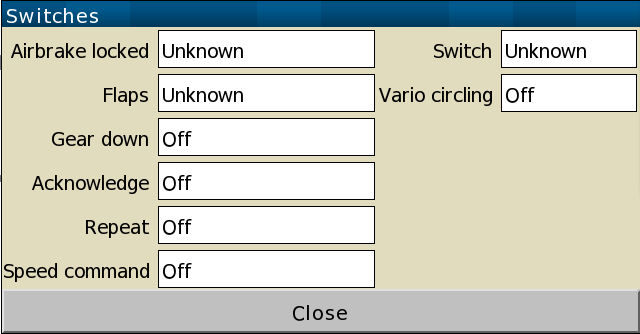
\includegraphics[angle=0,width=0.6\linewidth,keepaspectratio='true']{figures/dialog-switches.png}
\end{center}
%%%%%%%%%%%%%%%%%%%%%%%%%%%%%%%%%%%%%%%
\section{Slave Modus, Doppelsitzermodus,  Durchschleifen von Daten}\index{Slave-mode}\index{Dosi-Modus}

Einer der im NMEA-Anschluß Menü befindlichen Treiber (''NMEA-Output'') bietet den sog.\  ''Slave-Modus'', welcher verwendet werden kann,  um z.B. zwei Geräte  (\al oder \textsf{PDA})  im Master-Slave Modus miteinander zu verbinden. \menulabel{\bmenut{Konfig}{3/3}\blink\bmenut{NMEA}{Anschluss}} 

% Erreichbar ist dies unter %Bis V625
% \begin{quote}
% \smenus{Konfig.}\blink\smenus{Konfig.}\blink\smenut{System}{Einstellung}\blink\seite{15}
% \end{quote}
% Untermenü ''Treiber''

Im als Master definierten Gerät muß dazu der Treiber des zweiten Gerätes \menulabel{\button{Einstellung}\blink\button{NMEA-Anschluss}} (Gerät B) als NMEA-OUT gesetzt werden.

Hierdurch werden alle ein- und ausgehenden Datensätze  durchgeschleift und an das als Slave definierte Gerät weitergereicht.
Im Slave-Gerät muß dann als Gerät A z.B.\ \fl als Treiber angewählt werden.

Als Beispiel seien im linken Bild der Master, rechts der Slave dargestellt, welche von einem \fl gespeist werden.:


\begin{center}%ab V6.4
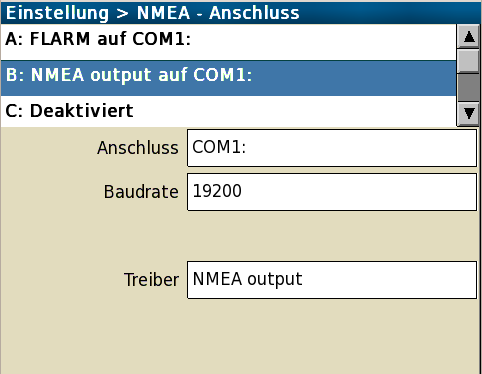
\includegraphics[angle=0,width=0.45\linewidth,keepaspectratio='true']{figures/config-nmea-ms-master.png}~~~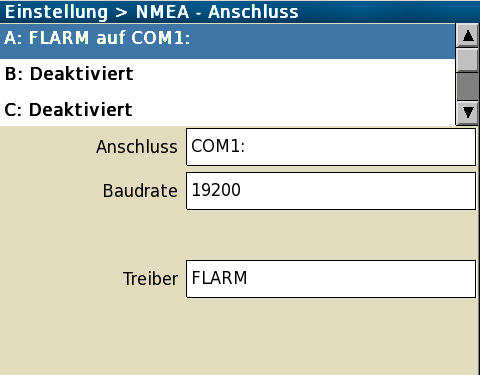
\includegraphics[angle=0,width=0.45\linewidth,keepaspectratio='true']{figures/config-nmea-ms-slave.png}
\end{center}

%\begin{center}% bis V 6.25
%\begin{tabbing}
%Anschluß\quad\=  COM1  hspace{10em}   \=  Anschluß\quad\=  COM1\kill
%\textbf{Master-Gerät:} \>             \> \textbf{Slave-Gerät:}\\[0.5em]
%\textsf{Gerät A}       \>             \> \textsf{Gerät A}\\
%Anschluß\quad\>  COM1  \>                Anschluß\quad\>  COM1\\
%Baudrate\> 19200       \>                Baudrate\> 19200\\
%Treiber                \>           \al\>                           Treiber\> \al\\[0.75em]
%
%\textsf{Gerät B}       \>                         \>  \textsf{Gerät B}\\
%Anschluß\>  COM2       \>           Anschluß\>  COM1\\
%Baudrate\> 19200       \>           Baudrate\> 19200\\
%Treiber\> NMEA OUT     \>           Treiber\> \textsl{beliebig}\\[0.75em]
%\end{tabbing}
%\end{center}



Auf diese Art und weise werden beide Geräte mit den identischen Daten versorgt, so, als ob sie direkt vom \fl, VEGA, o.ä.\ kämen. 
Auf gleiche Weise können zwei \al mit identischen Daten versorgt werden, wenn nur eine Datenquelle zur Verfügung steht.

Zur entsprechenden Verkabelung bitte die entsprechenden Handbücher der Geräte konsultieren.

%%%%%%%%%%%%%%%%%%%%%%%%%%%%%%%%%%%%%%%%%%%%%%%%%%55
\section{Systemstatus Dialog}\label{sec:system-status-dialog}\index{Status!System}\index{Status!Angeschlossene Geräte}\index{Status!Flug}

Der Systemstatus-Dialog (auch Kap.~\ref{sec:dialog-windows}) wird hauptsächlich zum Systemcheck benutzt und hier vor allem, ob die Verbindung zu den angeschlossenen Geräten voll etabliert und OK ist
%\begin{quote}
%\smenus{Info}\blink\smenus{Info}\blink\smenus{Status}
%\end{quote}
\menulabel{\bmenut{Info}{2/3}\blink\bmenus{Status}} In den weiteren Untermenüs \button{Flug}, \button{Aufgabe}, \button{Regeln} und \button{Zeiten} können entsprechende Daten abgeglichen werden. Diese Daten sind rein zur Information und können hier nicht editiert werden! 

%%%%%%%%%%%%%%%%%%%%%%%%%%%%%%%%%%
\section{Mehrere Verbindungen zu externen Geräten}\index{Externe Geräte}

Es können bis zu zwei externe Geräte konfiguriert werden, welche parallel angeschlossen und betrieben werden können. Einige \textsf{PDA} haben zwei serielle Schnittstellen, Verbindungen per Bluetooth können prinzipiell mehrere unabhängige Verbindung etablieren.

Wenn  beide Geräte GPS-Signale zur Verfügung stellen können, dann wird das primäre, erste Gerät von \xc ausgewählt und das zweite bleibt ignoriert. Sowie die erste GPS-Quelle aus irgendeinem Grunde versagt, wird automatisch auf die zweite Quelle umgeschaltet und zwar solange, bis die erste Quelle wieder gültige GPS-Daten übermittelt. (fallback)

Das gleiche gilt für alle Werte wie z.B. barometrische Höhe, Vario, Geschwindigkeit etc.\
\xc bevorzugt grundsätzlich das primäre Gerät, und greift auf das sekundäre Gerät zurück, sowie das Primäre versagt.

Beispielkonfiguration:
Primäres Gerät ist Cambridge CAI 302, das sekundäre Gerät sei \fl. Diese Kombination bietet von beiden Geräten das Beste
%%%%%%%%%%%%%%%%%%%%%%%%%%%%%%%%%%%%%%
\section{Verwaltung der angeschlossenen Geräte, NMEA-Anschluß etc.\ }\index{NMEA!Info}

Das NMEA-Ansichtsfenster ist wie folgt zu erreichen:
%\begin{quote}
%\smenus{Konfig}\blink\smenus{Konfig}\blink\smenus{Konfig}\blink\smenut{NMEA-}{Anschluß}\blink%bis 6.4
%\end{quote}

Hier können angeschlossene Geräte und  deren Ausgänge  betrachtet werden.\menulabel{\bmenut{Konfig}{2/3}\blink\bmenut{NMEA}{Anschluss}}

Der Button \button{Wiederverbinden} dient dazu, das gerät mit \xc neu wiederzuverbinden. Dies geschieht normalerweise automatisch, aber in manchen Fällen kann es sinnvoll sein, dies manuell zu versuchen - bspw.\ Fehlersuche\dots

Der Button \button{Flug Donwload} ist nur verfügbar, wenn ein IGC-Logger an \xc angeschlossen ist.  \ref{sec:supported-varios}
Wenn anklickt wird, erscheint eine Liste aufgezeichneter Flüge, welche entsprechend geladen werden kann.  Die Datei  wird geladen und in das \texttt{logs}-Unterverzeichnis des  \texttt{XCSorData } - Verzeichnis kopiert.

\button{Bearbeiten} ermöglicht die Bearbeitung der NMEA-Quellen und Anschlüsse

Der Button \button{Verwalten} ist nur dann verfügbar, wenn ein VEGA oder ein CAI 302 angeschlossen ist. Hier werden spezielle Eigenschaften dieser beiden Geräte unterstützt.  Bspw.\  das Löschen des Flugspeichers beim CAI 302. \warning Genau hier kann es Verzögerungen kommen, da teilweise ein Firmware-Fehler  des CAI 302 auftritt.

Mit \button{Überwachung} werden in Klartext die Ausgaben der angeschlossenen Geräte ausgegeben\footnote{Hoffe, das ist richtig so}. Sinnvoll zum Debuggen bzw.\ finden von Fehlern bei ''komischen'' GPS-Quellen.
%finished für v6.5 date 08/02/2013 OH





